% Drawing 138/04-3 -- folder 138, batch 04, archive page 63 (PDF page 64).
% Transcription: une double pyramide : sommet $E^{+}$ en haut, $E^{-}$ en bas ; à l'équateur le triangle $D_{20}$, $D_{01}$, $D_{12}$ (ce dernier en arrière). Les arêtes sont les applications $p^{\pm}_{20}$, $p^{\pm}_{01}$, $p^{\pm}_{12}$ de $E^{\pm}$ vers les $D_{ij}$. Sur les faces sont placés $S_0$, $S_1$, $S_2$, atteints par des flèches $\pi^{\pm}_0$, $\pi^{\pm}_1$, $\pi^{\pm}_2$ issues de $E^{\pm}$, et par des flèches $q_{02}\colon D_{20} \to S_0$, $q_{01}\colon D_{01} \to S_0$, $q_{20}$, $q_{10}$, $q_{12}$, $q_{21}$ issues des sommets de l'équateur.
% Kind: double pyramid (diagram of maps). Method 2 (schematic redraw from the facsimile). Status: partial.
% Notes: Double pyramid: E+ at the top, E- at the bottom, the equator triangle D_20, D_01 (front) and D_12 (back). The points S_0, S_1, S_2 are the midpoints of the three equator edges (D_20 D_01, D_12 D_01, D_20 D_12 on the page, to within a unit), so they are computed on those edges, and the arrows q_02, q_01, q_20, q_21, q_12, q_10 are the half-edges from the D_ij to them, each ending on the same S point (q_10 dashed). From E+ and from E-: p^pm_20 (solid) to D_20, p^pm_01 (solid) to D_01, p^pm_12 (dashed) to D_12, pi^pm_0 (solid) to S_0, pi^pm_1 and pi^pm_2 (dashed) to S_1 and S_2; every edge is drawn between the same vertex points. Labels as on the page. Still differs: his strokes are slightly curved and often stop short of the vertices, here they are straight and reach them; a second label read pi_1^+ beside the edge E+ D_01 near D_01 is set as read (it may be a rewritten p_01^+); the faint pencil construction lines crossing the upper half and the left (two long thin strokes towards D_12, one towards S_2) and his doublings of the edges are left out. The formulas rho_0^+ = ..., rho_1^+ = ..., rho_2^+ = ... at the right are text. Nothing is struck. Redrawn 2026-11-09 (issue 128): to check again. Overlay check 2026-11-14 (issue 147, Claude Opus 5.5): the redraw, rasterised from its TikZ paths, laid over the colour render of the 250 ppi scan with the contrast raised: the vertices, the solid and dashed edges and the arrowheads of the double pyramid lie on their ink to within about 1 unit, the labels on theirs. Nothing changed. Still differs, as listed above: his edges are slightly curved and stop short of the vertices where the redraw reaches them; the second label near D_01 is a reading; the faint pencil construction lines are left out. Not compiled (no TeX engine in the session).
% Coordinates: 1 unit = 1 mm = 1/100 of the crop width (bbox in page fractions: [0.17, 0.1, 0.53, 0.51]).
% Redrawn by Claude (claude-opus-5-5), issue #73, 2026-11-09; not checked by a human; not compiled (no TeX in the session).
% Checked by Claude (claude-opus-5-5) 2026-11-14 (issue #147): overlay on the 300 dpi colour render of the 250 ppi scan; nothing changed; not compiled (no TeX in the session). Not checked by a human. Status: partial.
% Rights: reproduces part of the work -- behind RENDER_TRANSCRIPTS, never published by itself.
\documentclass[tikz,border=3pt]{standalone}
\usepackage{amsmath,amssymb}
\usetikzlibrary{patterns,arrows.meta}
\tikzset{pencil/.style={black!45}, struck/.style={black!35}, mark/.style={circle,draw,inner sep=1.3pt}, pt/.style={circle,fill,inner sep=0.9pt}, opt/.style={circle,draw,fill=white,inner sep=1.1pt}}
\begin{document}
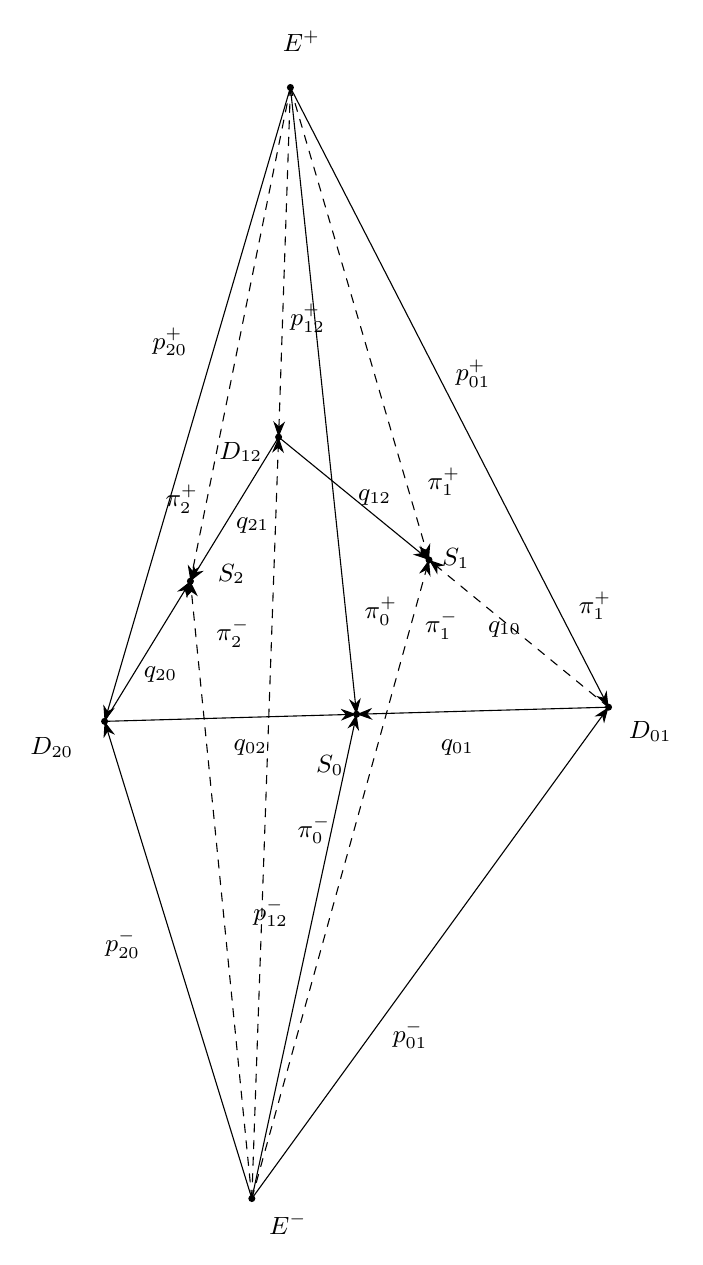
\begin{tikzpicture}[x=1mm,y=1mm,line cap=round,line join=round,font=\scriptsize]
\draw[-{Stealth[length=2mm]}] (47.3,-15.2) -- (23.7,-95.7);
\draw[dashed,-{Stealth[length=2mm]}] (47.3,-15.2) -- (34.6,-77.9);
\draw[dashed,-{Stealth[length=2mm]}] (47.3,-15.2) -- (45.8,-59.6);
\draw[-{Stealth[length=2mm]}] (47.3,-15.2) -- (55.7,-94.8);
\draw[dashed,-{Stealth[length=2mm]}] (47.3,-15.2) -- (64.9,-75.2);
\draw[-{Stealth[length=2mm]}] (47.3,-15.2) -- (87.7,-93.9);
\draw[-{Stealth[length=2mm]}] (42.4,-156.3) -- (23.7,-95.7);
\draw[dashed,-{Stealth[length=2mm]}] (42.4,-156.3) -- (34.6,-77.9);
\draw[dashed,-{Stealth[length=2mm]}] (42.4,-156.3) -- (45.8,-59.6);
\draw[-{Stealth[length=2mm]}] (42.4,-156.3) -- (55.7,-94.8);
\draw[dashed,-{Stealth[length=2mm]}] (42.4,-156.3) -- (64.9,-75.2);
\draw[-{Stealth[length=2mm]}] (42.4,-156.3) -- (87.7,-93.9);
\draw[-{Stealth[length=2mm]}] (23.7,-95.7) -- (55.7,-94.8);
\draw[-{Stealth[length=2mm]}] (87.7,-93.9) -- (55.7,-94.8);
\draw[-{Stealth[length=2mm]}] (23.7,-95.7) -- (34.6,-77.9);
\draw[-{Stealth[length=2mm]}] (45.8,-59.6) -- (34.6,-77.9);
\draw[-{Stealth[length=2mm]}] (45.8,-59.6) -- (64.9,-75.2);
\draw[dashed,-{Stealth[length=2mm]}] (87.7,-93.9) -- (64.9,-75.2);
\node[pt] at (47.3,-15.2) {};
\node[pt] at (42.4,-156.3) {};
\node[pt] at (23.7,-95.7) {};
\node[pt] at (87.7,-93.9) {};
\node[pt] at (45.8,-59.6) {};
\node[pt] at (55.7,-94.8) {};
\node[pt] at (64.9,-75.2) {};
\node[pt] at (34.6,-77.9) {};
\node[inner sep=1pt] at (48.7,-9.3) {\small $E^{+}$};
\node[inner sep=1pt] at (47,-159.5) {\small $E^{-}$};
\node[inner sep=1pt] at (17,-99) {\small $D_{20}$};
\node[inner sep=1pt] at (93,-97) {\small $D_{01}$};
\node[inner sep=1pt] at (41,-61.5) {\small $D_{12}$};
\node[inner sep=1pt] at (52.3,-101.3) {\small $S_0$};
\node[inner sep=1pt] at (68.3,-75) {\small $S_1$};
\node[inner sep=1pt] at (39.8,-77) {\small $S_2$};
\node[inner sep=1pt] at (32,-47.5) {\small $p^{+}_{20}$};
\node[inner sep=1pt] at (49.5,-44.5) {\small $p^{+}_{12}$};
\node[inner sep=1pt] at (70.5,-51.5) {\small $p^{+}_{01}$};
\node[inner sep=1pt] at (33.5,-67.5) {\small $\pi^{+}_{2}$};
\node[inner sep=1pt] at (66.8,-65.3) {\small $\pi^{+}_{1}$};
\node[inner sep=1pt] at (58.8,-81.7) {\small $\pi^{+}_{0}$};
\node[inner sep=1pt] at (86,-81) {\small $\pi^{+}_{1}$};
\node[inner sep=1pt] at (42.5,-70.8) {\small $q_{21}$};
\node[inner sep=1pt] at (58,-67.3) {\small $q_{12}$};
\node[inner sep=1pt] at (30.8,-89.8) {\small $q_{20}$};
\node[inner sep=1pt] at (42.2,-99) {\small $q_{02}$};
\node[inner sep=1pt] at (68.5,-99) {\small $q_{01}$};
\node[inner sep=1pt] at (74.5,-84) {\small $q_{10}$};
\node[inner sep=1pt] at (40,-84.5) {\small $\pi^{-}_{2}$};
\node[inner sep=1pt] at (66.5,-83.5) {\small $\pi^{-}_{1}$};
\node[inner sep=1pt] at (50.3,-109.5) {\small $\pi^{-}_{0}$};
\node[inner sep=1pt] at (26,-124) {\small $p^{-}_{20}$};
\node[inner sep=1pt] at (44.8,-120) {\small $p^{-}_{12}$};
\node[inner sep=1pt] at (62.5,-135.5) {\small $p^{-}_{01}$};
\end{tikzpicture}
\end{document}
